\section{Graphen}


Im Allgemeinen kann ein Graph durch $G = (V, E)$ dargestellt werden, wobei $V$ eine Menge an Knoten und $E$ eine Menge an Kanten ist. Die Kanten sind jeweils ein geordnetes Knotenpaar $(u, v) \subseteq V \times V$.

\subsection{Dichte}
\label{dichte}

Die Dichte eines Graphen gibt das Verhältnis zwischen der Anzahl an Kanten und der potentiell möglichen Anzahl an Kanten an \cite{diestel2010graphentheorie}.
Sie lässt sich bestimmen mit:

\[ d(G) =  \frac{2|{E}|}{|V|(|V| - 1)}    \]


\subsection{Knotengrad}
\label{knotengrad}

In einem gerichteten Graphen besitzt jeder Knoten einen Ausgang- und Eingangsgrad. Dies ist jeweils die Anzahl an Kanten, die bei dem Knoten starten bzw. bei ihm enden \cite{diestel2010graphentheorie}.
Der Ausgangsgrad für einen Knoten $v$ im Graph $G$ wird mit $d^{+}_{G}(v)$ und den Eingangsgrad mit $d^{-}_{G}(v)$ bezeichnet.


\subsection{Multi Layer Graphen}

Im Folgenden werden Multi Layer Graphen betrachtet. Diese Graphen haben neben Knoten und Kanten auch eine Menge an Ebenen. Dabei kann, je nach Art des Graphen, der gleiche Knoten in verschiedene Ebenen vorhanden sein oder auch Verbindungen zwischen den Knoten in verschiedenen Ebenen bestehen.
Welche Bedeutung den Ebenen zukommt, hängt vom Graphen und dem Anwendungsfall der Daten ab. Multi Layer Graphen können genutzt werden, um Netzwerke in unterschiedlichen Themengebieten abzubilden, z.B. soziale Netzwerke, Transport oder Biologie.

Multi Layer Graphen können, abhängig von ihren Verbindungen, in verschiedene Kategorien eingeteilt werden. Die verschiedenen Kategorien sind in Abbildung \ref{network_types} dargestellt. 

\begin{figure}
  \centering
  \begin{subfigure}[b]{1.0\textwidth}
    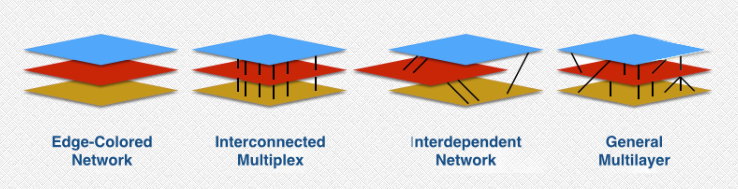
\includegraphics[width=1.0\linewidth]{img/network_types.png}
  \end{subfigure}
  \caption{Multi Layer Netzwerkarten \cite{muxVizBild}}
  \label{network_types}
\end{figure}

\subsubsection{Edge Colored Network}

In Edge Colored Networks gibt es nur Kanten zwischen Knoten im gleichen Layer. Dabei sind die Kanten jeweils mit einem Label versehen das kennzeichnet, zu welchem Layer sie gehören.


\subsubsection{Interconnected Multiplex}

In Multiplex Netzwerken gibt es hauptsächlich Kanten zwischen Knoten, die sich im gleichen Layer befinden. Die einzigen Kanten, die es zwischen verschiedenen Layern gibt, verbinden jeweils den gleichen Knoten in dem anderen Layer. 

\subsubsection{Inderdependet Network}

In Inderdependet Networks gibt es keine Knoten, die in mehr als einem Layer vorkommen. Kanten können Knoten innerhalb eines Layers, aber auch zwischen zwei Layern verbinden.

\subsubsection{Generelle Multi Layer}
In einem Generellen Multi Layer Graph gibt es keine Restriktion, wie die Knoten der verschiedene Ebenen miteinander verbunden sein können. Es kann sowohl Verbindungen zwischen dem gleichen Knoten in verschiedenen Ebenen geben, als auch Verbindungen zu Knoten in anderen Ebenen.


Ein genereller Multi Layer Graph kann formal als ein gerichteter Multigraph\cite{multiLayerMath} $G = (\Sigma_{V}, \Sigma_{E}, V, E, s, t, l_{V}, l_{E})$, dessen Knoten und Kanten ein Label besitzen, definiert werden, wo

\begin{itemize}
  \item V die Menge an Knoten und E die Menge an Kanten ist
  \item $\Sigma_{V}$ und $\Sigma_{E}$ die Alphabete sind, die als Label für Knoten und Kanten dienen
  \item $s: E \rightarrow V$ und $t: E \rightarrow V$ zwei Zuordnungen sind, die angeben, von welchem Knoten eine Kante ausgeht und zu welchem sie führt
  \item $l_{V}: V \rightarrow \Sigma_{V}$ und $l_{E}: V \rightarrow \Sigma_{E}$ zwei Zuordnungen sind, die den Knoten und Kanten ihre Labels zuweisen
\end{itemize}

Da mit den Generellen Multilayer Graphen auch alle anderen Arten von MultiLayer Graphen dargestellt werden können, werden im Folgendem nur noch Generelle Multigraphen betrachtet.
